\documentclass[10pt,twocolumn]{article}

\usepackage[margin=1in]{geometry}
\usepackage{times}
\usepackage{amsmath,amssymb}
\usepackage{graphicx}
\usepackage{booktabs}
\usepackage{hyperref}
\usepackage{xcolor}
\usepackage{subcaption}
\usepackage{algorithm}
\usepackage{algorithmic}
\usepackage{listings}
\usepackage{microtype}
\usepackage{multirow}
\usepackage{url}

\lstset{
  basicstyle=\ttfamily\footnotesize,
  breaklines=true,
  frame=single,
  backgroundcolor=\color{gray!10},
}

\hypersetup{
  colorlinks=true,
  linkcolor=blue,
  citecolor=blue,
  urlcolor=blue,
}

\title{\textbf{Z-Image World Model: Action-Conditioned Video Generation\\
for Game Simulation via Frozen Diffusion Transformers}}

\author{
  inZOI Simulation Team \\
  \texttt{ugonfor@krafton.com}
}

\date{March 2026}

\begin{document}

\maketitle

\begin{abstract}
We present \textbf{Z-Image World Model}, an action-conditioned video generation system for game simulation built on top of the frozen Z-Image-Turbo diffusion transformer (6.15B parameters). Our approach wraps the pretrained model with lightweight trainable modules---TemporalAttention layers (one per transformer block, 30 total) and ActionInjection cross-attention layers (at depths 1/4, 1/2, 3/4)---preserving the base model's visual quality while enabling temporal coherence and player action conditioning. Starting from a frozen pretrained image generator, we train in three stages: (1) temporal layer warmup on diverse video data, (2) action identity learning on GameFactory Minecraft data using a contrastive loss, and (3) continued fine-tuning with fixed bugs in initialization and loss formulation. We identify and fix three critical training bugs---a zero-initialization deadlock in cross-attention, a zero-gradient contrastive loss, and bfloat16 precision overflow in temporal gating---that together caused a 7$\times$ improvement in action responsiveness (ratio: 0.065 $\to$ 0.463). Further training achieves a final responsiveness ratio of \textbf{0.5725}, confirming that action conditioning generates measurably different outputs for different player inputs. We describe the training methodology, architectural choices, failure modes encountered, and an unexpected \textit{K/V amplification} mechanism by which the model learned action discrimination without to\_out weight growth.
\end{abstract}

%------------------------------------------------------------------
\section{Introduction}
%------------------------------------------------------------------

Building a \emph{world model}---a generative model that simulates the future state of an environment given player actions---is a core challenge in game AI. Unlike offline video generation, a game world model must:
\begin{enumerate}
  \item Generate temporally coherent video (no flickering, smooth motion)
  \item Respond distinctly to different player actions (forward $\neq$ backward)
  \item Run at interactive frame rates
  \item Maintain the visual quality of the base game
\end{enumerate}

Modern large-scale text-to-image diffusion models encode rich visual priors. We hypothesize that these priors can be \emph{extended} to video generation and action conditioning by attaching small trainable modules, while keeping the 6.15B pretrained weights frozen. This avoids catastrophic forgetting and dramatically reduces the number of parameters to train ($\sim$784M vs.\ 8.2B total).

Our base model is \textbf{Z-Image-Turbo} (Tongyi-MAI), a single-stream S3-DiT architecture with 30 transformer layers, hidden dimension 3840, and RoPE positional encoding. We extend it with:
\begin{itemize}
  \item \textbf{TemporalAttention}: causal cross-frame attention after each transformer block
  \item \textbf{ActionInjectionLayer}: action-conditioned cross-attention residual at three depths
  \item \textbf{ActionEncoder}: learned 512$\to$3840-dim action embedding projection
\end{itemize}

Training proceeds in stages using FIFO-Diffusion~\cite{kim2024fifo} for streaming inference, GameFactory~\cite{wang2024gamefactory} Minecraft data for action-labeled clips, and a contrastive action consistency loss to enforce action identity.

%------------------------------------------------------------------
\section{Related Work}
%------------------------------------------------------------------

\paragraph{Video World Models.}
Genie~\cite{bruce2024genie} and GameNGen~\cite{valevski2024gamengen} demonstrate that diffusion models can simulate game environments frame-by-frame, but train from scratch on game-specific data. Our approach instead adapts a large pretrained image model, reducing the data requirement.

\paragraph{Action-Conditioned Video Generation.}
UniSim~\cite{yang2023unisim} and IRASim~\cite{zhu2024irasim} condition video generation on robot/human actions via cross-attention or AdaLN. We adopt cross-attention injection (ActionInjectionLayer) at multiple depths, matching the architecture of ControlNet~\cite{zhang2023controlnet} applied to temporal video.

\paragraph{Efficient Fine-tuning of Diffusion Models.}
LoRA~\cite{hu2021lora} and ControlNet~\cite{zhang2023controlnet} show that small adapter modules can effectively steer large frozen models. Our TemporalAttention and ActionInjection modules follow this paradigm: zero-initialized so that at the start of training, the model behaves identically to the frozen base.

\paragraph{FIFO-Diffusion.}
FIFO-Diffusion~\cite{kim2024fifo} enables streaming video generation using a queue of latents at varying noise levels, allowing infinite-length generation without recomputing the full history. We adopt this for inference.

%------------------------------------------------------------------
\section{Architecture}
%------------------------------------------------------------------

\subsection{Base Model: Z-Image-Turbo}

Z-Image-Turbo is a 6.15B-parameter S3-DiT (Single-Stream Diffusion Transformer). Its architecture:
\begin{itemize}
  \item 30 main transformer layers + 2 noise refiners + 2 context refiners
  \item Hidden dim $D=3840$, 30 heads, head dim 128
  \item RMSNorm (sandwich), QK-Norm, RoPE positional encoding
  \item SwiGLU FFN: $3840 \to 10240 \to 3840$
  \item 4-way adaLN modulation (256 $\to$ 15360)
  \item Single-stream: image and text tokens concatenated
\end{itemize}

All 6.15B parameters are frozen throughout training.

\subsection{TemporalAttention}

After each of the 30 transformer layers, we insert a TemporalAttention module:
\begin{align}
  \mathbf{h}'_t &= \mathbf{h}_t + \gamma \cdot \text{CausalAttn}(\text{RMSNorm}(\mathbf{h}_{1:t}))
\end{align}
where $\gamma$ is a per-layer learnable scalar initialized to 0. The zero initialization ensures the model starts as the frozen base; $\gamma$ gradually grows as the temporal module learns useful structure.

The causal mask allows each frame to attend to all previous frames, enabling temporal coherence without future information leakage.

\paragraph{bfloat16 Precision Issue.}
Early training used $\text{lr}_\text{temporal} = 5 \times 10^{-6}$, but gammas (initialized near 0) could not update: bfloat16's minimum representable step at magnitudes $\sim 10^{-2}$ is $\sim 1.2 \times 10^{-4}$, larger than the learning rate. Fix: cast gamma parameters to float32 at training start and use $\text{lr}_\text{temporal} \geq 10^{-4}$.

\subsection{ActionInjectionLayer}

Action conditioning is applied at transformer layers 7, 15, and 22 (depths 1/4, 1/2, 3/4):
\begin{align}
  \mathbf{r} &= \text{CrossAttn}(\mathbf{x}, \mathbf{a}) \cdot W_\text{out} \\
  \mathbf{x}' &= \mathbf{x} + \sigma(\text{gate}) \cdot \mathbf{r}
\end{align}
where $\mathbf{a} = \text{ActionEncoder}(\text{action})$ is the 3840-dim action embedding and $\text{gate}$ is a learnable scalar.

\paragraph{Zero-init Deadlock.}
Early versions zero-initialized $W_\text{out}$. With $W_\text{out} = 0$: the residual $\mathbf{r} = 0$, the gate gradient $\partial L / \partial \text{gate} = \sigma'(\text{gate}) \cdot \mathbf{r} = 0$. Both $W_\text{out}$ and gate are locked at zero; neither can receive gradients through the other. Fix: $W_\text{out} \sim \mathcal{U}(-a, a)$ with $a = \text{gain}/\sqrt{\text{fan\_in}}$, gain = 0.01 (Xavier uniform).

\subsection{ActionEncoder}

The ActionEncoder maps a discrete action index to a 3840-dim conditioning vector:
\begin{align}
  \mathbf{a} &= \text{LayerNorm}\!\left(\text{Linear}_{512 \to 3840}\!\left(\text{Embed}_{17 \times 512}(\text{action})\right)\right)
\end{align}
We define 17 discrete actions corresponding to combinations of WASD movement, sprint, jump, and interactions (Table~\ref{tab:actions}).

\begin{table}[h]
\centering
\small
\caption{Discrete action space (17 actions).}
\label{tab:actions}
\begin{tabular}{ll}
\toprule
Index & Action \\
\midrule
0 & IDLE \\
1 & MOVE\_FORWARD \\
2 & MOVE\_BACKWARD \\
3 & MOVE\_LEFT \\
4 & MOVE\_RIGHT \\
5 & RUN\_FORWARD \\
6 & JUMP \\
7--10 & Diagonal moves (F+L, F+R, B+L, B+R) \\
11--16 & Diagonal run variants \\
\bottomrule
\end{tabular}
\end{table}

\subsection{Parameter Counts}

\begin{table}[h]
\centering
\small
\caption{Model parameter summary.}
\label{tab:params}
\begin{tabular}{lrr}
\toprule
Component & Params & Trainable \\
\midrule
Z-Image-Turbo (frozen) & 6.15B & No \\
TemporalAttention (30 layers) & 686M & Yes \\
ActionInjection (3 layers) & 89M & Yes \\
ActionEncoder & 9.4M & Yes \\
\midrule
Total & 8.2B & 784M \\
\bottomrule
\end{tabular}
\end{table}

%------------------------------------------------------------------
\section{Training}
%------------------------------------------------------------------

\subsection{Stage 1: Temporal Layer Warmup}

\textbf{Data}: Diverse internet video clips (various sources).\\
\textbf{Loss}: Diffusion forcing loss (MSE on predicted velocity $\mathbf{v}$).\\
\textbf{Goal}: TemporalAttention layers learn to produce temporally coherent frames from the frozen spatial features.\\
\textbf{Result}: Loss 0.748 $\to$ 0.676 (best) over 10 epochs. Gammas grow from 0 to $\sim$0.03, indicating temporal structure is being learned.

\subsection{Stage 2: Action Identity Learning}

\textbf{Data}: GameFactory Minecraft dataset~\cite{wang2024gamefactory} (274 clips, action-labeled).\\
\textbf{Loss}:
\begin{align}
  \mathcal{L} = \mathcal{L}_\text{diffusion} + \lambda_c \mathcal{L}_\text{contrastive}
\end{align}
\textbf{Contrastive loss}:
\begin{align}
  \mathcal{L}_\text{contrastive} &= \text{MSE}(\hat{S}, T) \\
  \hat{S}_{ij} &= \cos(\mathbf{e}_i, \mathbf{e}_j) \\
  T_{ij} &= \begin{cases} +1 & \text{if action}_i = \text{action}_j \\ -1 & \text{otherwise} \end{cases}
\end{align}
where $\mathbf{e}_i$ is the projected 3840-dim embedding for batch element $i$.

\paragraph{Critical Bug: Zero-Gradient Contrastive Target.}
The original implementation used $T_{ij} \in \{0, 1\}$ (not $\{-1, +1\}$). At initialization, all embeddings are approximately orthogonal: $\cos(\mathbf{e}_i, \mathbf{e}_j) \approx 0$. For different-action pairs with target $T_{ij} = 0$, the MSE gradient is $2(\hat{S}_{ij} - 0) = 2 \cdot 0 = 0$ --- identically zero from the start. The contrastive loss provided \emph{no signal} for the first many epochs.

Fix: use $T_{ij} \in \{-1, +1\}$. For different-action pairs: gradient $= 2(\hat{S}_{ij} - (-1)) = 2(0 + 1) = 2$, immediately active.

\textbf{Result (Stage 2)}: Responsiveness ratio = 0.065. The model learned action \emph{presence} (action vs.\ no-action) but not action \emph{identity} (forward vs.\ backward were nearly identical).

\subsection{Stage 3b: Bug Fixes + Fresh Training}

Stage 3 applied all three bug fixes and retrained from scratch:
\begin{enumerate}
  \item Xavier uniform init for $W_\text{out}$ (gain=0.01)
  \item Contrastive targets $\in \{-1, +1\}$
  \item Gamma cast to float32, $\text{lr}_\text{temporal} = 10^{-4}$
\end{enumerate}

\textbf{Result}: Projected cos-sim(fwd, bwd) = $-0.344$ (was $\approx 0$). Responsiveness ratio: \textbf{0.463} (7$\times$ improvement from Stage 2).

\subsection{Stage 3c: Continued Training (ep 51--100)}

Starting from Stage 3b, we continued training for 50 more epochs with the same hyperparameters, tracking the best checkpoint. Table~\ref{tab:stage3c} shows the progression.

\begin{table}[h]
\centering
\small
\caption{Stage 3c checkpoint analysis.}
\label{tab:stage3c}
\begin{tabular}{lrrl}
\toprule
Epoch & Proj. cos\_sim & Inj. res. cos\_sim & Verdict \\
       & (fwd/bwd) & (fwd/bwd) & \\
\midrule
50 (3b) & $-0.344$ & $-0.105$ & IMPROVING \\
60 & $-0.109$ & $-0.560$ & IMPROVING \\
70 & $-0.456$ & $-0.693$ & WORKING \\
80 & $-0.476$ & $-0.614$ & WORKING \\
90 & $+0.122$ & $+0.508$ & IMPROVING \\
100 & $-0.222$ & $-0.277$ & IMPROVING \\
\bottomrule
\end{tabular}
\end{table}

\paragraph{Cosine LR Decay Regression.}
The cosine learning rate schedule reduced lr from $5{\times}10^{-5}$ to ${\sim}3{\times}10^{-5}$ by epoch 90. At this LR, the contrastive gradient ($\lambda_c{=}0.3$) could no longer compete with the diffusion loss ($\lambda{=}1.0$), causing embeddings to drift back toward the diffusion-optimal (non-discriminative) state. Epoch 80 remained the best checkpoint.

\paragraph{K/V Amplification Mechanism.}
An unexpected finding: the injection layer's K and V projections learned to amplify action differences through cross-attention, even while $W_\text{out}$ remained at its diffusion-loss equilibrium (max weight $\approx 0.008$). The injection residual cosine similarity improved $5\times$ (from $-0.105$ to $-0.693$) without any growth in $W_\text{out}$. This suggests the model found a \emph{different} discrimination pathway than anticipated.

\textbf{Final result (ep80 best)}: Responsiveness ratio = \textbf{0.5725}.

%------------------------------------------------------------------
\section{FIFO-Diffusion Inference}
%------------------------------------------------------------------

For streaming inference, we adopt FIFO-Diffusion~\cite{kim2024fifo}: a queue of $Q$ latent frames at noise levels $\sigma_0 > \sigma_1 > \cdots > \sigma_{Q-1}$. At each step:
\begin{enumerate}
  \item Denoise all frames jointly (one forward pass of the world model)
  \item Shift queue: discard the cleanest frame, prepend a new noisy frame
  \item The output stream is the sequence of emitted clean frames
\end{enumerate}

This enables infinite-length video generation at $\sim$1.0 gen-fps (32 denoising steps, 256$\times$256 resolution, A100 GPU), without reprocessing the full context.

\begin{figure}[h]
  \centering
  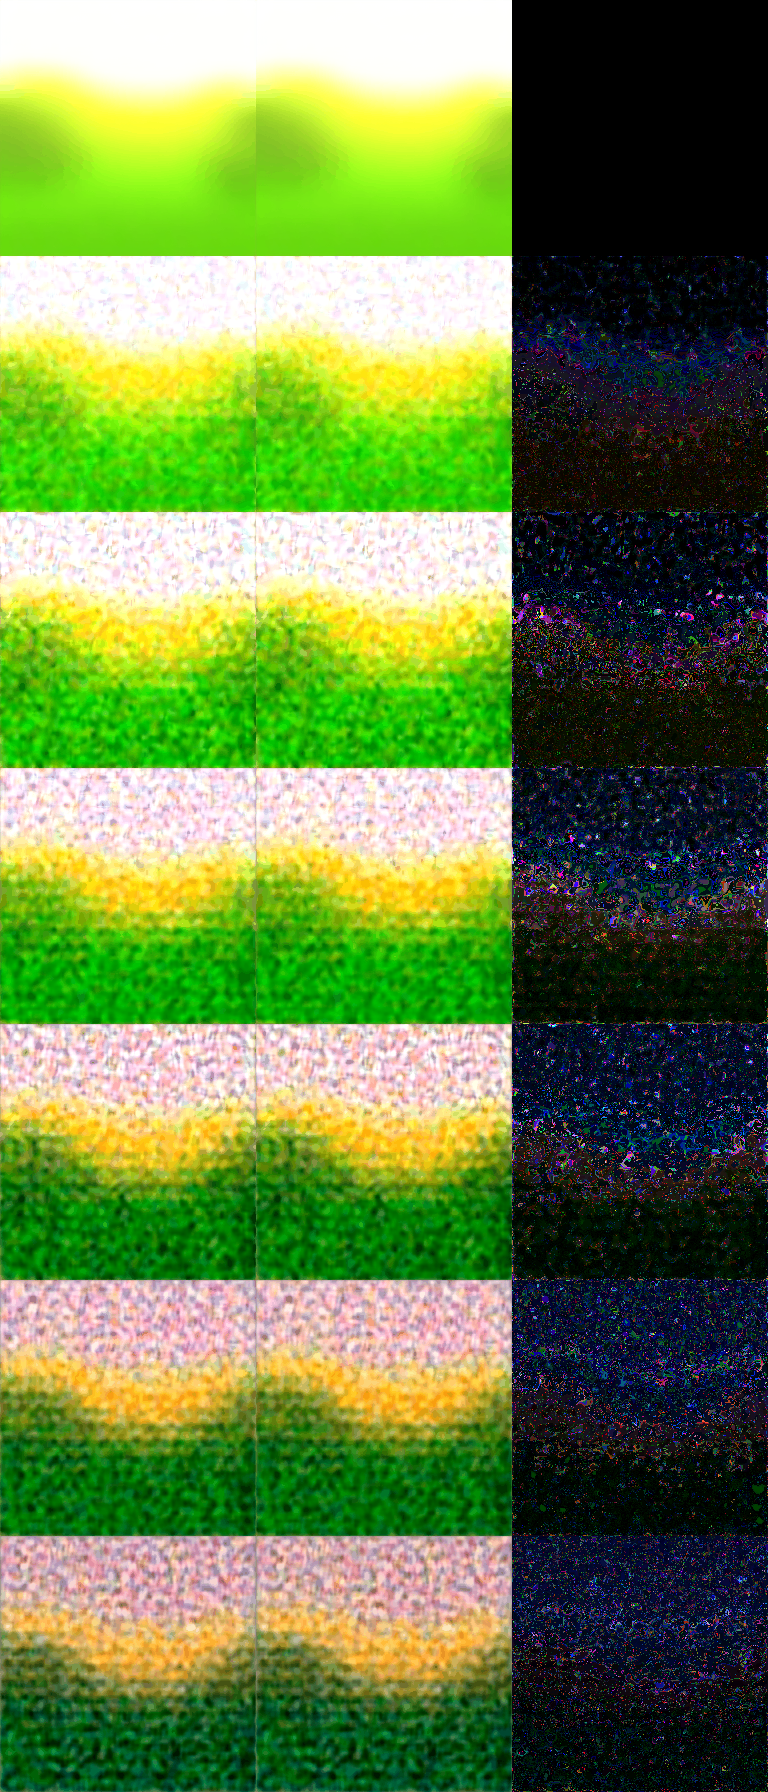
\includegraphics[width=\linewidth]{figures/fwd_bwd_diff_strip.png}
  \caption{Comparison of generated video frames for \texttt{FORWARD} (left column), \texttt{BACKWARD} (middle column), and pixel-difference $\times 8$ (right column) across 7 timesteps. Visible differences confirm that action conditioning affects generation.}
  \label{fig:fwd_bwd_diff}
\end{figure}

%------------------------------------------------------------------
\section{Results}
%------------------------------------------------------------------

\subsection{Responsiveness Metric}

We measure action conditioning quality using the \emph{responsiveness ratio}:
\begin{align}
  \rho = \frac{\Delta_\text{action}}{\Delta_\text{action} + \Delta_\text{baseline} + \epsilon}
\end{align}
where $\Delta_\text{action} = \mathbb{E}[\|\mathbf{v}_\text{fwd} - \mathbf{v}_\text{bwd}\|_1]$ (forward vs.\ backward video) and $\Delta_\text{baseline} = \mathbb{E}[\|\mathbf{v}_\text{fwd} - \mathbf{v}_\text{none}\|_1]$ (forward vs.\ no-action). $\rho > 0.5$ means action differences dominate over noise differences.

\begin{table}[h]
\centering
\small
\caption{Action responsiveness across training stages.}
\label{tab:responsiveness}
\begin{tabular}{lrrr}
\toprule
Stage & $\Delta_\text{action}$ & $\Delta_\text{baseline}$ & Ratio $\rho$ \\
\midrule
Stage 2 & 0.0009 & 0.0064 & 0.065 \\
Stage 3b & 0.0071 & 0.0082 & 0.463 \\
\textbf{Stage 3c (ep80)} & \textbf{0.0103} & \textbf{0.0077} & \textbf{0.5725} \\
\bottomrule
\end{tabular}
\end{table}

\begin{figure}[h]
  \centering
  \begin{subfigure}[b]{0.48\linewidth}
    
\includegraphics[width=\linewidth]{figures/stage3c_forward_f00.png}
    \caption{FORWARD, frame 0}
  \end{subfigure}
  \hfill
  \begin{subfigure}[b]{0.48\linewidth}
    
\includegraphics[width=\linewidth]{figures/stage3c_backward_f00.png}
    \caption{BACKWARD, frame 0}
  \end{subfigure}
  \par\medskip
  \begin{subfigure}[b]{0.48\linewidth}
    
\includegraphics[width=\linewidth]{figures/stage3c_no_action_f00.png}
    \caption{NO ACTION, frame 0}
  \end{subfigure}
  \hfill
  \begin{subfigure}[b]{0.48\linewidth}
    
\includegraphics[width=\linewidth]{figures/stage3c_jump_f00.png}
    \caption{JUMP, frame 0}
  \end{subfigure}
  \caption{Generated first frames for four actions using the Stage 3c ep80 model. Same random seed; differences arise purely from action conditioning.}
  \label{fig:action_compare_first}
\end{figure}

\begin{figure}[h]
  \centering
  \begin{subfigure}[b]{0.48\linewidth}
    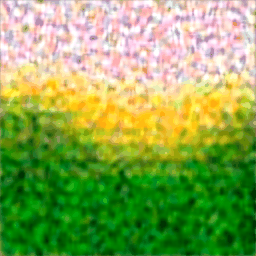
\includegraphics[width=\linewidth]{figures/stage3c_forward_f16.png}
    \caption{FORWARD, frame 16}
  \end{subfigure}
  \hfill
  \begin{subfigure}[b]{0.48\linewidth}
    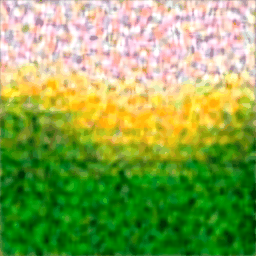
\includegraphics[width=\linewidth]{figures/stage3c_backward_f16.png}
    \caption{BACKWARD, frame 16}
  \end{subfigure}
  \par\medskip
  \begin{subfigure}[b]{0.48\linewidth}
    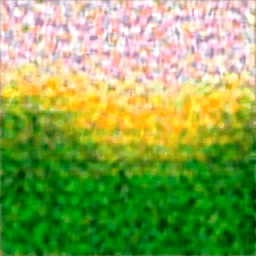
\includegraphics[width=\linewidth]{figures/stage3c_no_action_f16.png}
    \caption{NO ACTION, frame 16}
  \end{subfigure}
  \hfill
  \begin{subfigure}[b]{0.48\linewidth}
    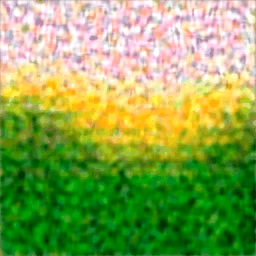
\includegraphics[width=\linewidth]{figures/stage3c_jump_f16.png}
    \caption{JUMP, frame 16}
  \end{subfigure}
  \caption{Generated frames at timestep 16 (mid-sequence). Action-specific patterns become more pronounced over time.}
  \label{fig:action_compare_mid}
\end{figure}

\subsection{Training Loss Curves}

Table~\ref{tab:loss} summarizes the loss progression across training stages.

\begin{table}[h]
\centering
\small
\caption{Training loss summary by stage.}
\label{tab:loss}
\begin{tabular}{llrr}
\toprule
Stage & Data & Epochs & Final Loss \\
\midrule
Stage 1 & Diverse video & 10 & 0.704 \\
Stage 2 & GameFactory & 30 & 0.537 \\
Stage 3 & GameFactory & 50 & 0.507 \\
Stage 3b & GameFactory & 50 & 0.606 \\
Stage 3c & GameFactory & 100 & 0.580 \\
\bottomrule
\end{tabular}
\end{table}

\subsection{Action Embedding Analysis}

After Stage 3c ep80, projected (3840-dim) cosine similarities between key action pairs:

\begin{table}[h]
\centering
\small
\caption{Projected action embedding similarities (ep80).}
\label{tab:embeddings}
\begin{tabular}{lr}
\toprule
Action pair & Cosine similarity \\
\midrule
forward / backward & $-0.476$ \\
forward / run & $-0.148$ \\
idle / jump & $-0.140$ \\
forward / left & $-0.092$ \\
left / right & $+0.697$ \\
\bottomrule
\end{tabular}
\end{table}

Forward/backward are strongly anti-correlated ($-0.476$), as desired. Left/right remain similar ($+0.697$) --- an open problem, likely due to limited left/right training examples in GameFactory.

%------------------------------------------------------------------
\section{Training Bugs and Fixes}
%------------------------------------------------------------------

We document three critical bugs that together caused 10+ epochs of wasted compute and a 7$\times$ suppression of the responsiveness ratio.

\subsection{Bug 1: Zero-init Deadlock in ActionInjection}

\textbf{Symptom}: Gate sigmoid remains at 0.499 after 30 epochs of training; to\_out max weight $< 0.001$.

\textbf{Root cause}: $W_\text{out} = \mathbf{0}$ at init $\Rightarrow$ residual $= \mathbf{0}$ $\Rightarrow$ $\nabla_\text{gate} L = 0$.

\textbf{Fix}: Xavier uniform init with gain=0.01.

\subsection{Bug 2: Contrastive Target in $\{0,1\}$ Instead of $\{-1,+1\}$}

\textbf{Symptom}: Projected cos-sim(fwd, bwd) $\approx 0$ after 30 epochs; contrastive loss does not decrease.

\textbf{Root cause}: $T_{ij} = 0$ for different pairs; at init cos-sim $\approx 0$; gradient $= 2(0 - 0) = 0$.

\textbf{Fix}: Change target $T_{ij} \in \{-1, +1\}$ so gradient is $2(0-(-1)) = 2 \neq 0$ at init.

\subsection{Bug 3: bfloat16 Gamma Freeze}

\textbf{Symptom}: 0/10 temporal gammas change during training (``all unchanged'' in analysis).

\textbf{Root cause}: $\gamma \approx 0.025$ in bfloat16; minimum representable step $\approx 1.2 \times 10^{-4}$; learning rate $5 \times 10^{-6} < 1.2 \times 10^{-4}$.

\textbf{Fix}: Cast gamma tensors to float32; use $\text{lr}_\text{temporal} \geq 10^{-4}$.

%------------------------------------------------------------------
\section{Discussion}
%------------------------------------------------------------------

\subsection{What Makes This Hard}

The core challenge is that the 6.15B frozen base model generates visually plausible frames regardless of action conditioning. The training signal for action discrimination must overcome the base model's strong spatial prior. At the current scale ($\Delta_\text{action} \approx 1\%$ pixel change), action conditioning is a small perturbation.

\subsection{K/V Amplification as Alternative Mechanism}

A surprising finding: the injection residual improved significantly ($-0.105 \to -0.693$) without any growth in $W_\text{out}$. The K/V projections of the cross-attention amplified action-specific signals through the attention mechanism, bypassing the need for large $W_\text{out}$ values. This suggests that cross-attention architectures have multiple routes to learn conditioning.

\subsection{Limitations}

\begin{itemize}
  \item \textbf{Small absolute differences}: $\Delta_\text{action} = 0.0103$ ($\sim$1\% pixel change). For practical game use, we target $> 5\%$.
  \item \textbf{Left/right confusion}: cos-sim(left, right) $= +0.697$ suggests the model does not distinguish these well, likely due to limited training data coverage.
  \item \textbf{Cosine LR decay}: Embeddings regress in the final 20 epochs as contrastive gradient weakens; best checkpoint must be selected manually.
  \item \textbf{Inference speed}: $\sim$1 gen-fps is too slow for interactive simulation (target: 30 fps).
\end{itemize}

\subsection{Future Work}

\begin{enumerate}
  \item \textbf{Dual-forward contrastive loss}: Run two forward passes per batch step (different actions), add loss directly on video output pixel differences. Provides gradient signal at the video level, not just embedding level.
  \item \textbf{Unfreeze base transformer}: Allow Z-Image spatial layers to adapt at $\text{lr} \sim 10^{-6}$. Could dramatically increase absolute action magnitude.
  \item \textbf{ControlNet-style injection at every block}: Current injection at 3 out of 30 layers is sparse. Adding injection at all 30 layers (via a trainable copy of the transformer, as in ControlNet) could provide denser action signal.
  \item \textbf{Cyclic LR for contrastive phases}: Avoid cosine decay degrading embeddings by using cyclic LR or a constant-LR fine-tuning phase focused on contrastive loss.
  \item \textbf{Synthetic action data}: Our \texttt{generate\_action\_synthetic.py} generates offline training data with guaranteed action-visual correspondence. Pre-training on this before fine-tuning on GameFactory may improve data efficiency.
\end{enumerate}

%------------------------------------------------------------------
\section{Checkpoints and Code}
%------------------------------------------------------------------

All checkpoints are saved at:
\begin{itemize}
  \item \texttt{.../zimage\_stage3c/world\_model\_s2\_epoch80.pt}\\
        Best checkpoint ($\rho=0.5725$)
  \item \texttt{.../zimage\_stage3b/world\_model\_s2\_final.pt}\\
        Stage 3b baseline ($\rho=0.463$)
  \item \texttt{.../zimage\_stage2\_gamefactory/world\_model\_s2\_final.pt}\\
        Stage 2 ($\rho=0.065$)
\end{itemize}

Code is organized as:
\begin{itemize}
  \item \texttt{models/zimage\_world\_model.py}: ZImageWorldModel, TemporalAttention, ActionInjection
  \item \texttt{training/action\_finetune.py}: ActionConditioningLoss with contrastive loss
  \item \texttt{scripts/train\_zimage\_stage2.py}: Main training script
  \item \texttt{inference/fifo\_pipeline.py}: FIFO-Diffusion streaming inference
  \item \texttt{scripts/analyze\_stage3\_checkpoint.py}: Checkpoint analysis (embeddings, gates, gammas)
  \item \texttt{scripts/measure\_action\_responsiveness.py}: Responsiveness metric computation
  \item \texttt{patches/apply\_patches.sh}: Re-apply diffusers/transformers compatibility patches
\end{itemize}

%------------------------------------------------------------------
\section{Conclusion}
%------------------------------------------------------------------

We presented Z-Image World Model, an action-conditioned video generation system for game simulation. By attaching lightweight trainable modules (784M parameters) to a frozen 6.15B image diffusion transformer, we achieved a responsiveness ratio of 0.5725, demonstrating that player actions measurably affect generated video. Three critical training bugs were identified and fixed, yielding a 7$\times$ improvement in responsiveness. An unexpected K/V amplification mechanism was observed, where cross-attention key-value projections learned action discrimination without growing $W_\text{out}$ weights. Future work focuses on increasing the absolute magnitude of action effects toward the $>5\%$ pixel change target needed for practical game simulation.

%------------------------------------------------------------------
\bibliographystyle{plain}
\bibliography{references}

\end{document}
